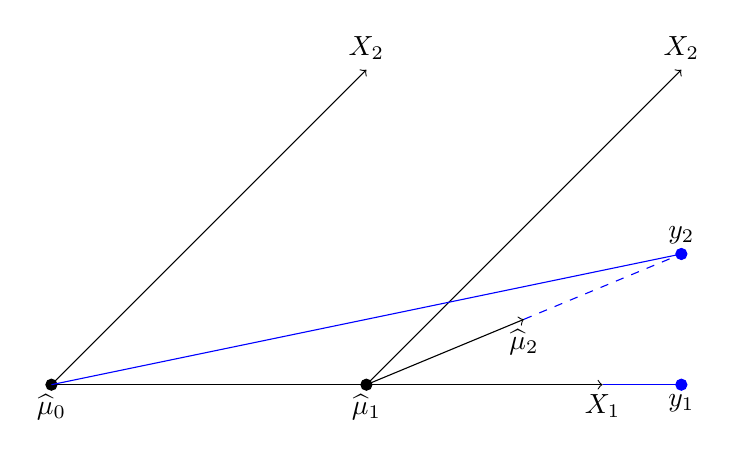
\begin{tikzpicture}
\draw [<-] (4,0) node [below] {$X_1$}-- (-3,0);
\filldraw (1,0) circle (2pt) node [below] {$\widehat{\mu}_1$};
\filldraw (-3,0)  circle (2pt) node [below]{$\widehat{\mu}_0$};
\draw [<-] (5,4) node [above] {$X_2$} --(1,0);
\draw [<-] (1,4) node [above] {$X_2$} --(-3,0);

\draw [blue](5,1.66)  node [above, black] {$y_2$} -- (-3,0);

\draw [->](1,0) -- (3, 0.83)  node [below] {$\widehat{\mu}_2$} ;
\draw [dashed, blue] (3,0.83) -- (5,1.66) ; 


\filldraw [blue] (5,1.66) circle (2pt) ;
\draw [blue]  (5,0) node [below] {} -- (4,0);
\filldraw [blue] (5,0) circle (2pt) ;
\draw (5,0) node [black, below] {$y_1$};
\end{tikzpicture}